\subsection{シミュレータ}
NEURONは,Yale大学のHinesらによって開発されている神経回路・細胞シミュレーションソフトウェアであり,
神経回路シミュレーションにおいて標準の一つとなっており,先行研究としてあげた宮本らによる
手動での高速化においても対象となったソフトウェアである. そのため,本研究の目的である神経回路シミュレーションの自動最適化の
対象としてNEURONを採用した. また,京やクラスタといった複数の計算機上で安定して稼働させるためにNEURONのバージョンは7.2を選択した.\\

\subsubsection{全体構成}
NEURONでは,MODファイルとHOCファイルと呼ばれる二つのファイルに必要な情報を記述することで神経回路シミュレーションを行っている.\\
MODファイルはその名のとおり神経細胞のモデルを記述するファイルであり, ( TODO : 章番号)で示したように神経細胞を数理モデルとして記述する.\\
一方でHOCファイルと呼ばれるファイルにはMODファイルで記述された神経細胞モデル間のつながりや,
シミュレーション時間などシミュレーションそのものに関与する設定を記述する.\\
より具体的には,図 ( TODO: 番号)で示したように,nrnivmodlと呼ばれるトランスパイラによってMODファイルは対応するCファイルに変換される.
このCファイルはさらにGCCやICCといったC言語のコンパイラによってオブジェクトファイルになり,ここで生成されたオブジェクトファイルと
NEURON本体がリンクされることによってNEURONの実行形式が作成されることになる.
そのため,MODファイルとして利用者が作成したモデルは実行時にはNEURONに組み込まれていることとなる.\\
最終的にこうして生成されたNEURONの実行形式に対してシミュレーションの情報を記述したHOCファイルを渡すことでシミュレーションが実行される.\\
\begin{figure}[htb]
% h:here, t:top, b:bottom, p:page
  \begin{center}
    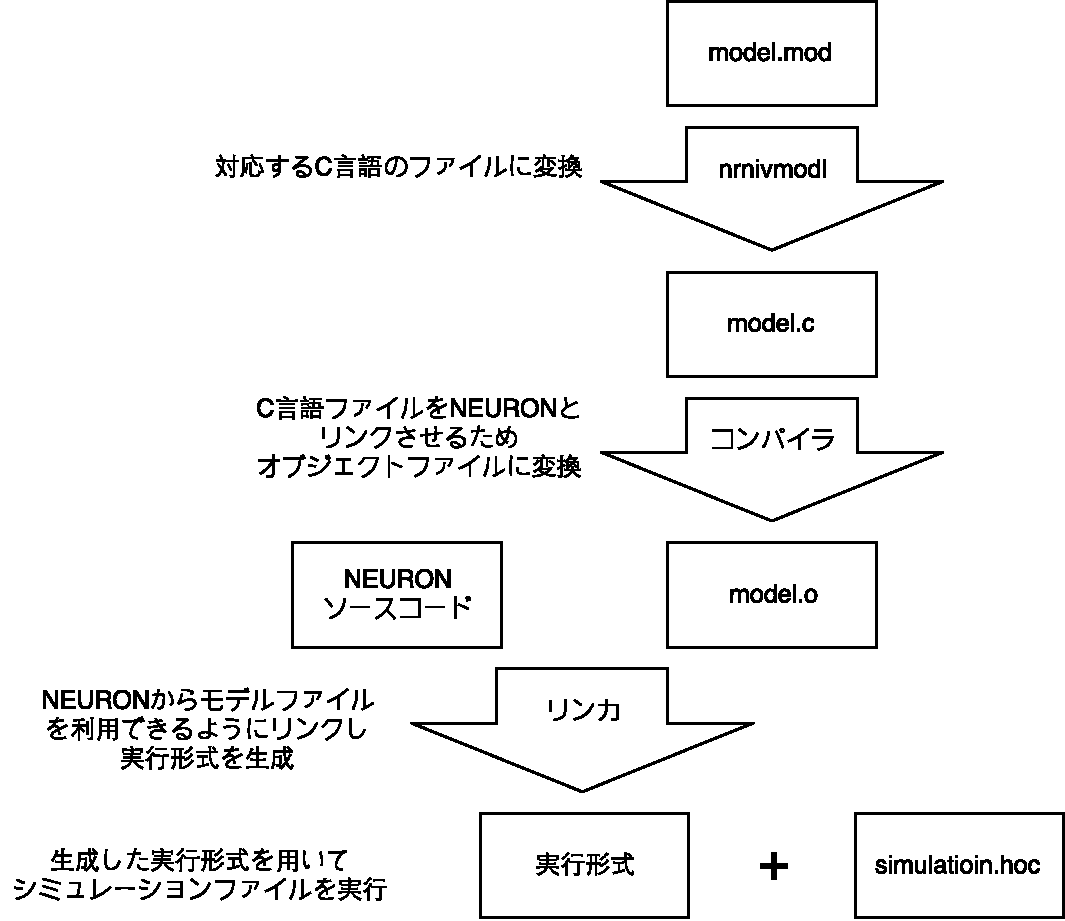
\includegraphics[width=10.0cm, angle=-90]{./images/neuron}
    \caption{NEURONの全体構成}
    \label{fig:neuron}
  \end{center}
\end{figure}~\\
宮本らによる先行研究では,主にこのMODファイルからCファイルへの変換に着目し,nrnivmodlによって作成されたCファイルを手動にて
最適化することでシミュレーション全体の高速化を達成した.\\
そのため,本研究においてはnrnivmodlに変わるトランスパイラを作成し自動での高速化を図る.\\

\subsubsection{NEURONのコンパイル}
\paragraph{クラスタ上でのコンパイル}~\\
( TODO: 宮本さんのから引用)
一般のx86環境では,
{\footnotesize
\begin{lstlisting}[caption=クラスタでのNEURONのコンパイル,label=cluster-neuron-compile,numbers=none]
$ ./configure --prefix=`pwd`\
              --without-iv --without-x --without-nrnoc-x11
$ make
$ make install
\end{lstlisting}
}
とすることでNEURONをコンパイルし,実行形式を得ることができる.
また,NEURONはデフォルトではGUI関係のライブラリもリンクするが,クラスタ上では必要ないためオプションを渡すことで
コンパイル対象から除外している.\\
\paragraph{京上でのコンパイル}~\\
( TODO: 宮本さんのから引用)
一方で,京ではログインノードと呼ばれるNEURONのコンパイルを行う環境(x86)とプログラムを実行する環境(sparc64)が
異なるため,クロスコンパイルを行う必要がある.\\
NEURONのコンパイルは内部的には
1. MODコンパイラ(nmodl)をコンパイルし実行形式を生成
2. MODコンパイラがMODファイルをC言語ファイルに変換した上でコンパイル
3. NEURON本体(nrniv, nrnoc)をコンパイルする
4. 上述の2と3をリンクさせ,実行形式を作成
という手順を踏んでいるが,この中でMODコンパイラ作成についてはログインノード(x86)で実行する必要があるため,1については
ネイティブコンパイルで,2,3,4についてはクロスコンパイルで行う必要がある.\\
またGUI関係のライブラリについてはクラスタ同様京でも必要ないため,除外する\\
\subparagraph{nmodlのコンパイル}~\\
{\footnotesize
\begin{lstlisting}[caption=京でのnmodlのコンパイル,label=k-nmodl-compile,numbers=none]
$ ./configure --prefix=`pwd`\
              --without-iv --without-x --without-nrnoc-x11\
              --with-nmodl-only linux_nrnmech=no\
              CC=gcc CXX=g++
$ make
$ make install
\end{lstlisting}
}
\subparagraph{NEURONのクロスコンパイル}
NEURON本体をクロスコンパイルする前に, 上述したnmodlのコンパイルで生成した実行形式をPATHの通っているディレクトリに
移動させておく必要がある. nmodlを退避させたのち,下記のコマンドを実行することでNEURON本体の実行形式が生成される
{\footnotesize
\begin{lstlisting}[caption=京でのNEURON本体のコンパイル,label=k-neuron-compile,numbers=none]
$ make clean
$ ./configure --prefix=`pwd`\
              --without-x --without-nmodl\
              --host=sparc64-unknown-linux-gnu --build=x86_64-unknown-linux-gnu\
              --without-iv --without-nrnoc-x11\
              --enable-shared=no --enable-static=yes\
              --with-paranrn --with-mpi --with-multisend\
              linux_nrnmech=no use_pthread=no\
              CC=mpifccpx CXX=mpiFCCpx MPICC=mpifccpx MPICXX=mpiFCCpx
$ make
$ make install
\end{lstlisting}
}

\subsubsection{NMODLについて}
本研究ではMODファイルを変換する
